%!TEX root = ../NCVC7.tex
\mysection{荒加工用のNCデータを生成}

\subsection{IGESデータの読み込み}
 図~\ref{fig:sample.iges} のIGESデータをNCVCで読み込みます.
この時点で \ref{sec:AboutIGES}~節にも書いたようにNCVCが落ちる場合があります.
IGESタイプを変更するなど適宜対応してください.

\begin{figure}[H]
\centering
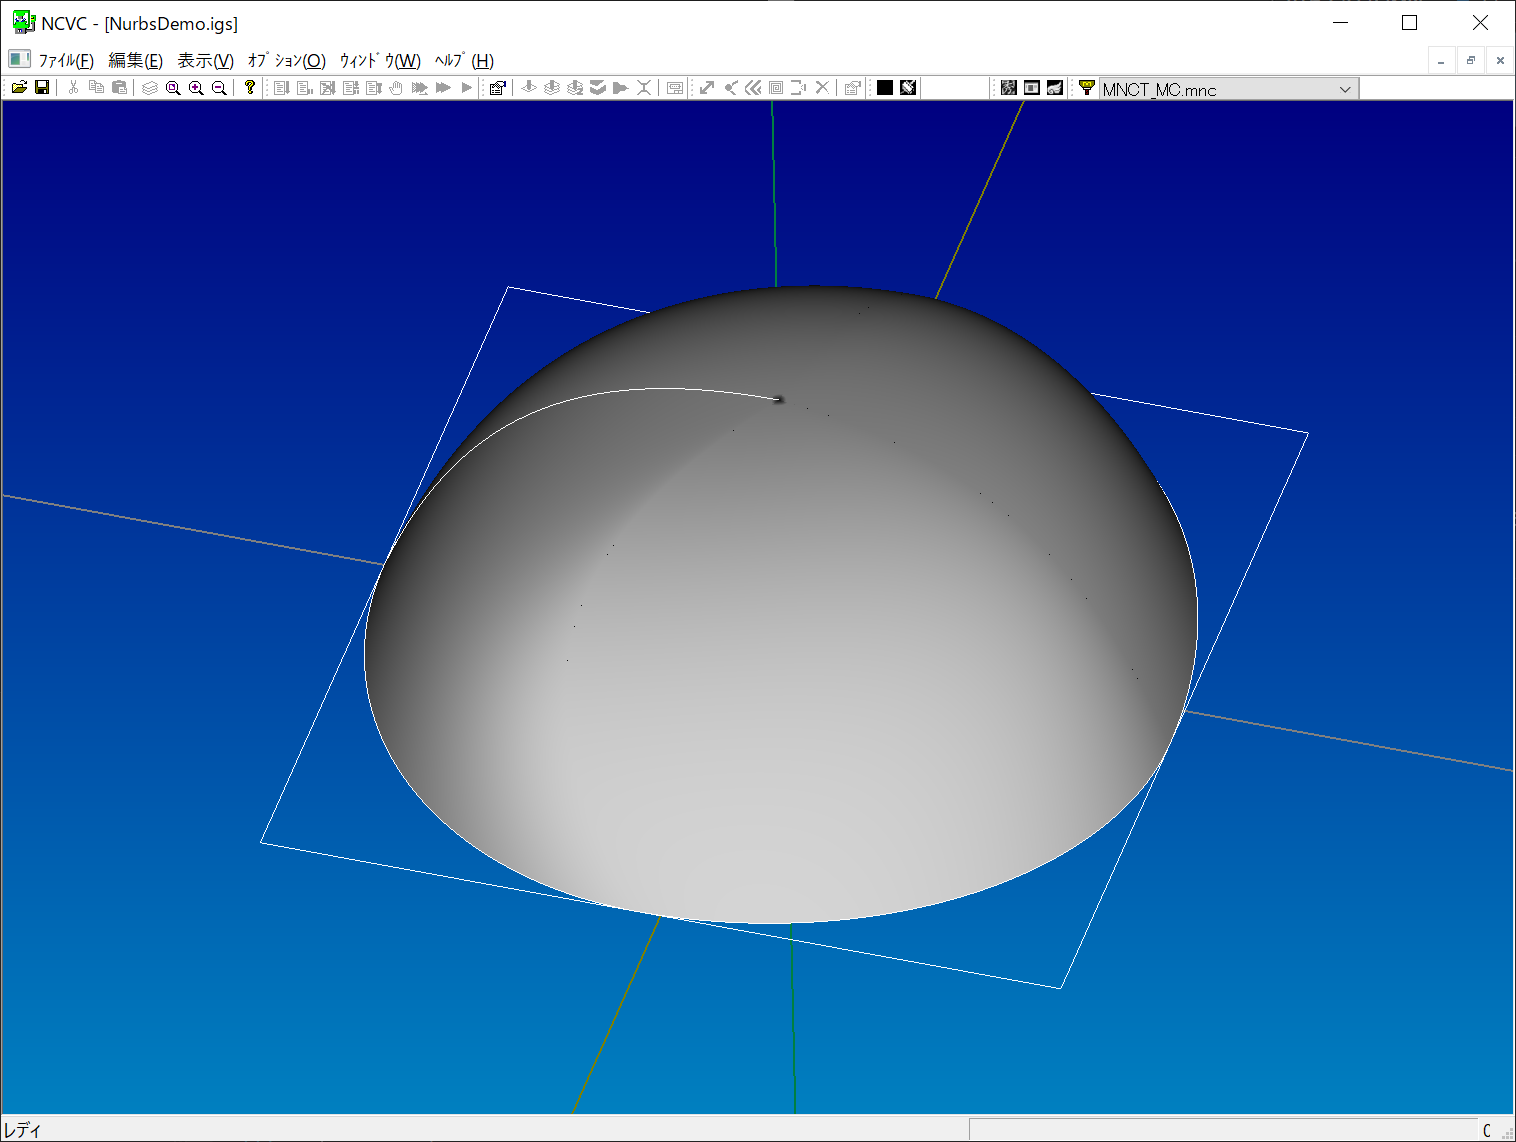
\includegraphics[scale=0.5]{No2/fig/fig21.png}
\caption{サンプル図形の読み込み}
\label{fig:ncvc21}
\end{figure}

\subsection{荒加工用スキャニングパスの生成}
 荒加工用のデータを生成するには,切削対象となる1つのNURBS曲面と,ガイドとなる1つのNURBS曲線を選択する必要があります.
マウスの左クリックで選択してください.選択順は問いません.
選択できると選択色
\footnote{\menu{オプション>表示属性>表示属性の設定}から\menu{共通}タブの\menu{選択オブジェクト}の色}
に変わります.

\begin{figure}[H]
\centering
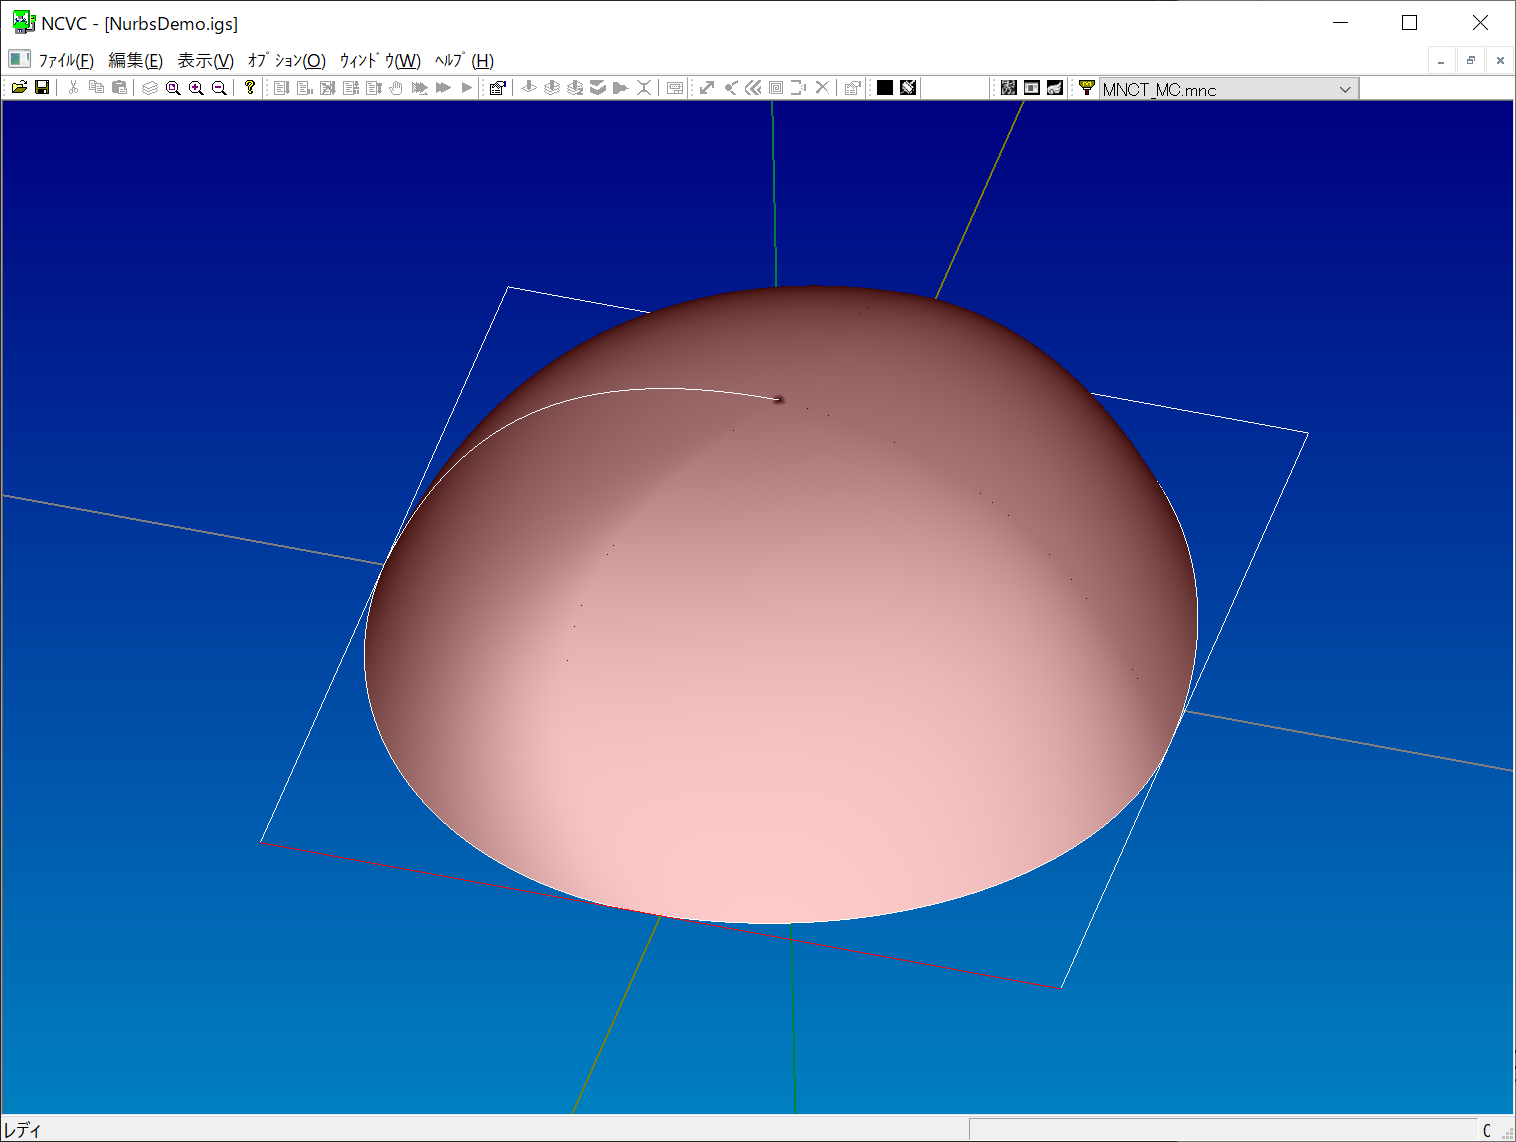
\includegraphics[scale=0.5]{No2/fig/fig22.png}
\caption{NURBS曲面とNURBS曲線の選択}
\label{fig:ncvc22}
\end{figure}

 NURBS曲面とNURBS曲線を選択すると,\menu{ファイル>NCデータの生成>荒加工パスの生成}(\keys{F2})のメニューが有効になります.
図~\ref{fig:ncvc23} のダイアログから適当な値を設定してください.

 [NC生成時,ワーク上面をZ軸のゼロにする]にチェックが入っていると[ワークの高さ]で設定した高さがZ軸のゼロになるようにNCデータが生成されます.
ワークの上面でZ軸の原点や工具長補正を設定する場合がほとんどだと思うので,通常はチェックを入れておきましょう.

\begin{figure}[H]
\centering
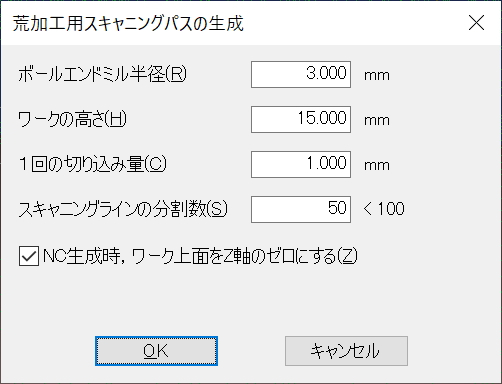
\includegraphics{No2/fig/fig23.png}
\caption{荒加工スキャニング設定}
\label{fig:ncvc23}
\end{figure}

 図~\ref{fig:ncvc23} で \keys{OK} を押すと,しばらく計算したあと,図~\ref{fig:ncvc24} のように荒加工パスが表示されます.
選択されたガイド曲線が[スキャニングラインの分割数]で分割され,さらにそのガイド曲線に沿うように点群が生成されます.

\begin{figure}[H]
\centering
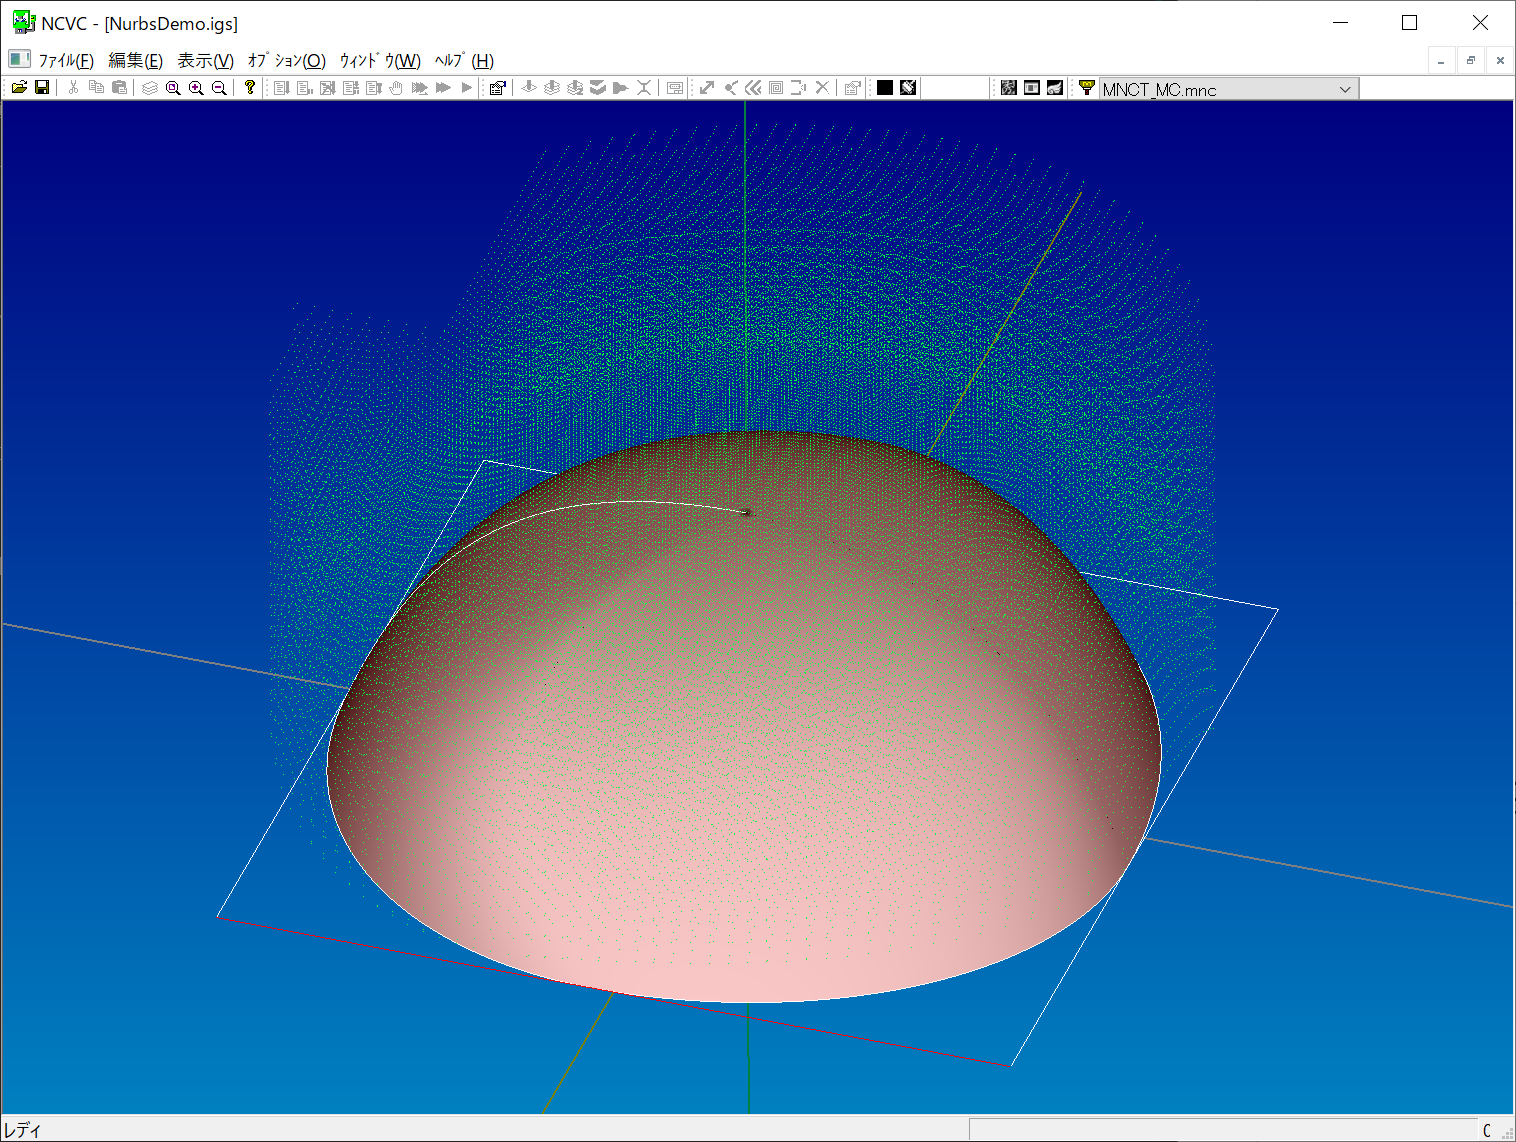
\includegraphics[scale=0.5]{No2/fig/fig24.png}
\caption{荒加工スキャニングパスの表示Ⅰ}
\label{fig:ncvc24}
\end{figure}

 図~\ref{fig:ncvc22} ではモデルの手前にあるX軸と平行なガイド曲線を選択したので,点群は図~\ref{fig:ncvc24} のようにY方向の集まりになりますが,
モデルの右(または左)側にあるY軸と平行なガイド曲線を選択すると,図~\ref{fig:ncvc25} のように点群はX方向の集まりになります.
\textbf{どちら方向に切削するかは,このガイド曲線の選択によって変わります.}

\begin{figure}[H]
\centering
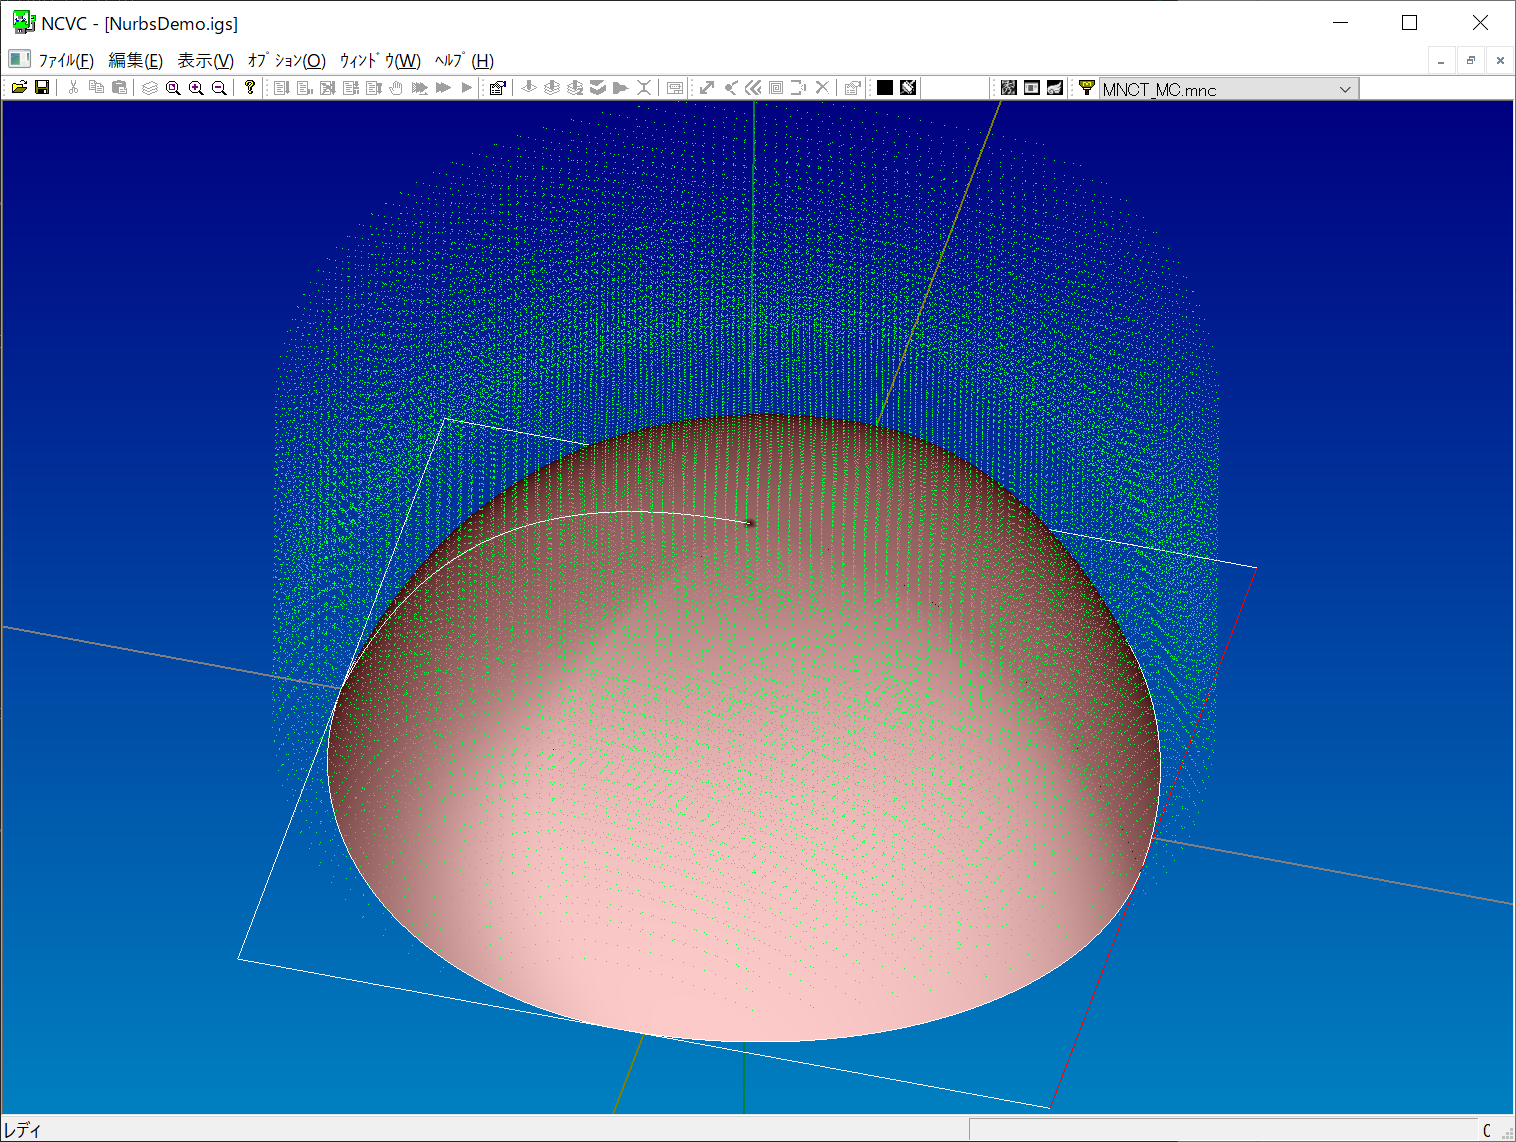
\includegraphics[scale=0.5]{No2/fig/fig25.png}
\caption{荒加工スキャニングパスの表示Ⅱ}
\label{fig:ncvc25}
\end{figure}

\subsection{NCデータの出力}
 \menu{ファイル>NCデータの生成>3D切削データの生成}(\keys{F7})のメニューから出力できます.
出力ファイル名にはデフォルトで荒加工用の \_Rough というサフィックス(接尾語)が付けられます(図~\ref{fig:ncvc26}).

 切削条件は2D切削と共通ですが,誤解のないように不要なタブは非表示にされています(図~\ref{fig:ncvc27}).
切削条件ファイルの拡張子(.nci)が共通というだけなので,3D切削用に設定しなおし,それ用に新規で保存しておきましょう.
カスタムヘッダー等も同様です.

\begin{minipage}{0.5\textwidth}
\begin{figure}[H]
\centering
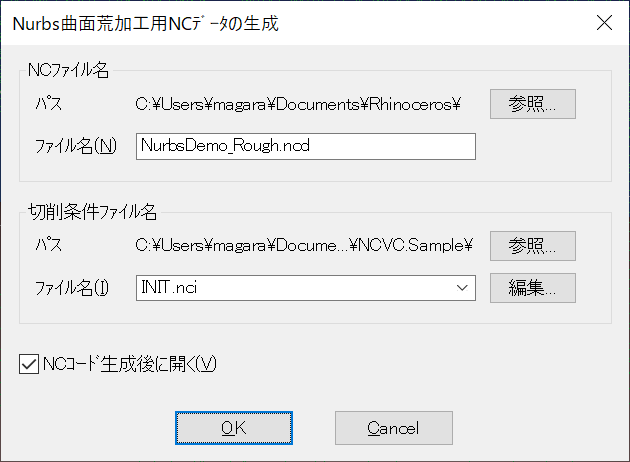
\includegraphics[scale=0.7]{No2/fig/fig26.png}
\caption{NCデータの出力設定}
\label{fig:ncvc26}
\end{figure}
\end{minipage}
\begin{minipage}{0.5\textwidth}
\begin{figure}[H]
\centering
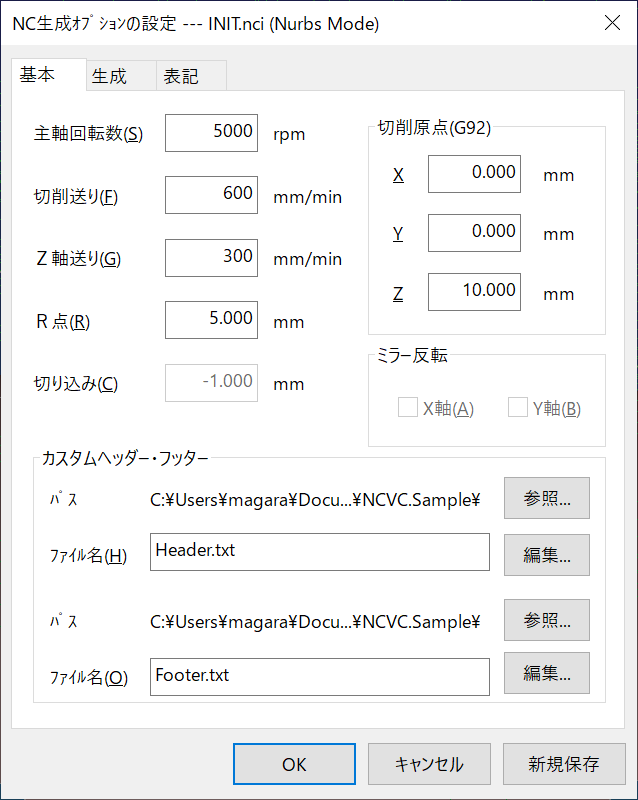
\includegraphics[scale=0.7]{No2/fig/fig27.png}
\caption{NURBS用の切削条件設定}
\label{fig:ncvc27}
\end{figure}
\end{minipage}

\vspace*{2zh}
 カスタムヘッダーも3D切削用に書き換えてください.
G92での原点指示は小型加工機に多い設定方法ですが,
ワーク座標系と工具長補正で設定を行う大型加工機の場合は,リスト~\ref{lst:header.txt} の方が一般的かもしれません.
ほか工具交換のGコード挿入など,積極的にカスタマイズしてください.

\begin{lstlisting}[caption=カスタムヘッダーの例,numbers=none,label=lst:header.txt]
%
G90G54G00X0Y0  → G92は削除  G54ワーク座標系のXY原点に移動
{Spindle}M03
G43Z50.H01     → 工具長補正でZ50.0まで移動
\end{lstlisting}

\subsection{NCデータのシミュレーション結果}
 図~\ref{fig:ncvc23} で指定したボールエンドミル半径が,NCVC用のOpenGL表示コメント

\vspace*{0.5zh}
\begin{breakbox}
\vspace*{-0.25cm}
\small
\begin{alltt}
(Endmill=R_)
\end{alltt}
\vspace*{-0.1cm}
\end{breakbox}

としてカスタムヘッダーの "\%" の次の行に挿入されます.
最大矩形はNCデータから自動算出されるので,図~\ref{fig:ncvc29} のように,ほぼ正確な切削イメージがシミュレーションできます.

 実はこのIGESデータで荒加工用のスキャニングパスを生成すると,\ref{sec:KodatunoMsg}~節の警告メッセージが出力されます.
そのせいで変なくぼみができてしまいました.
この対応については現在検討中です.

\begin{figure}[H]
\centering
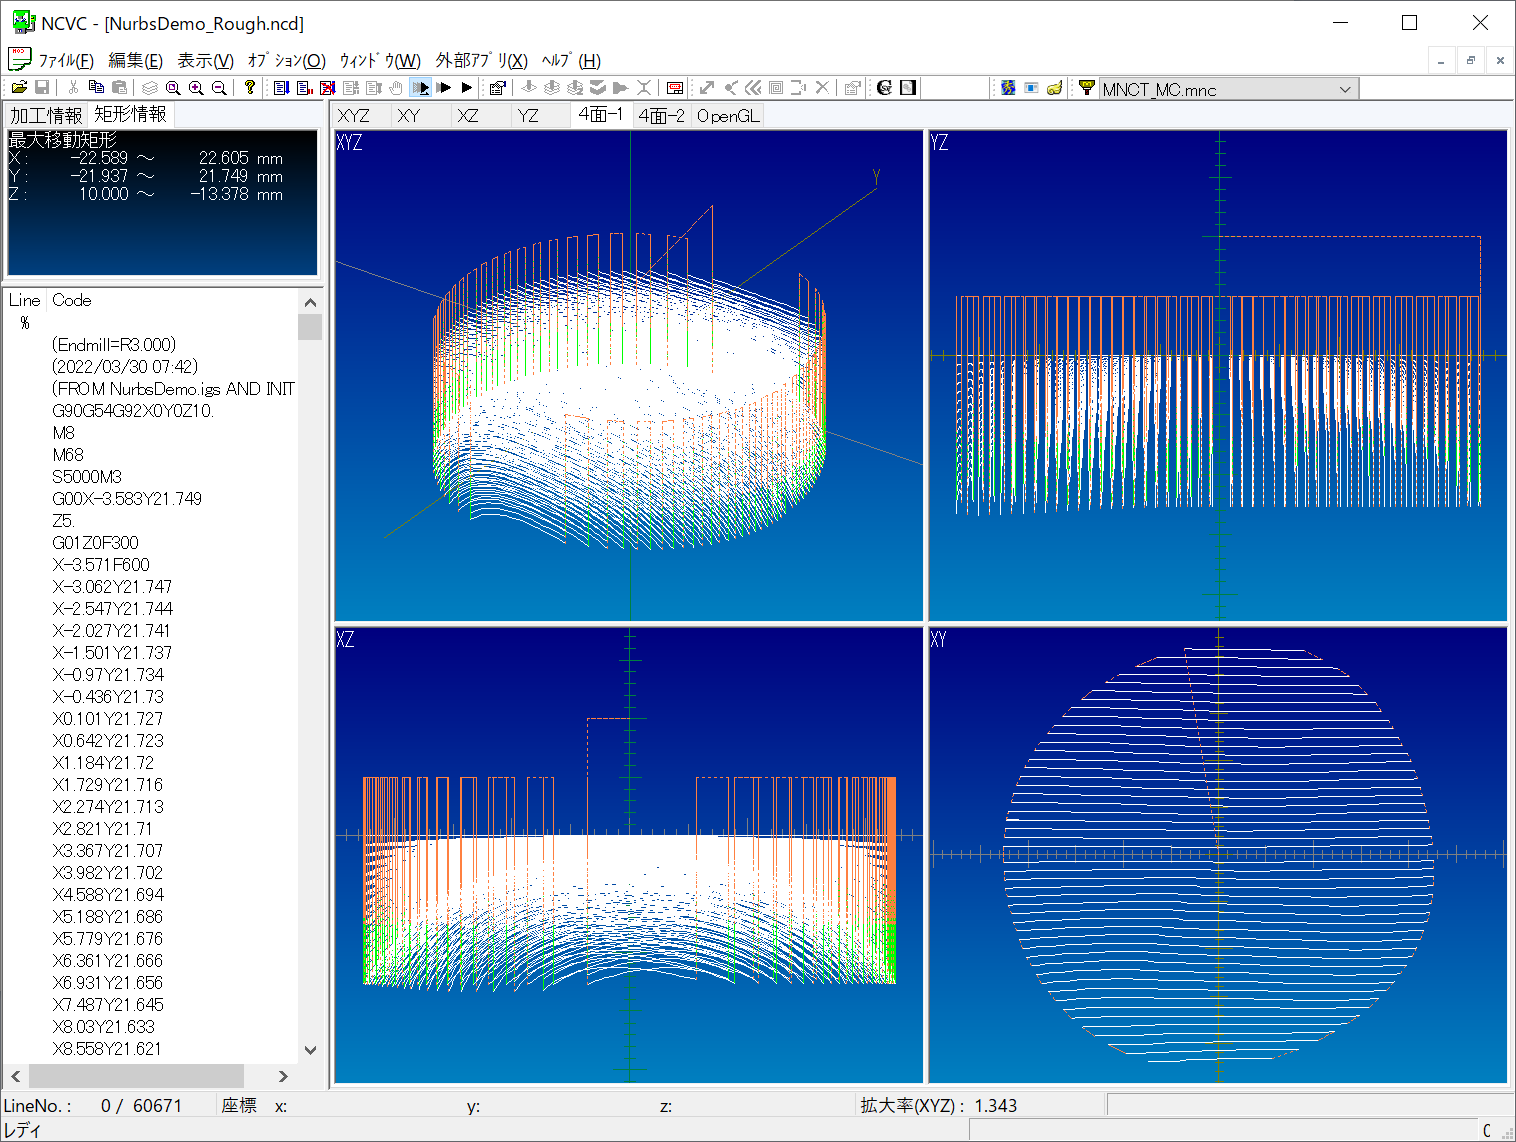
\includegraphics[scale=0.5]{No2/fig/fig28.png}
\caption{荒加工NCデータのシミュレーション結果Ⅰ}
\label{fig:ncvc28}
\end{figure}

\begin{figure}[H]
\centering
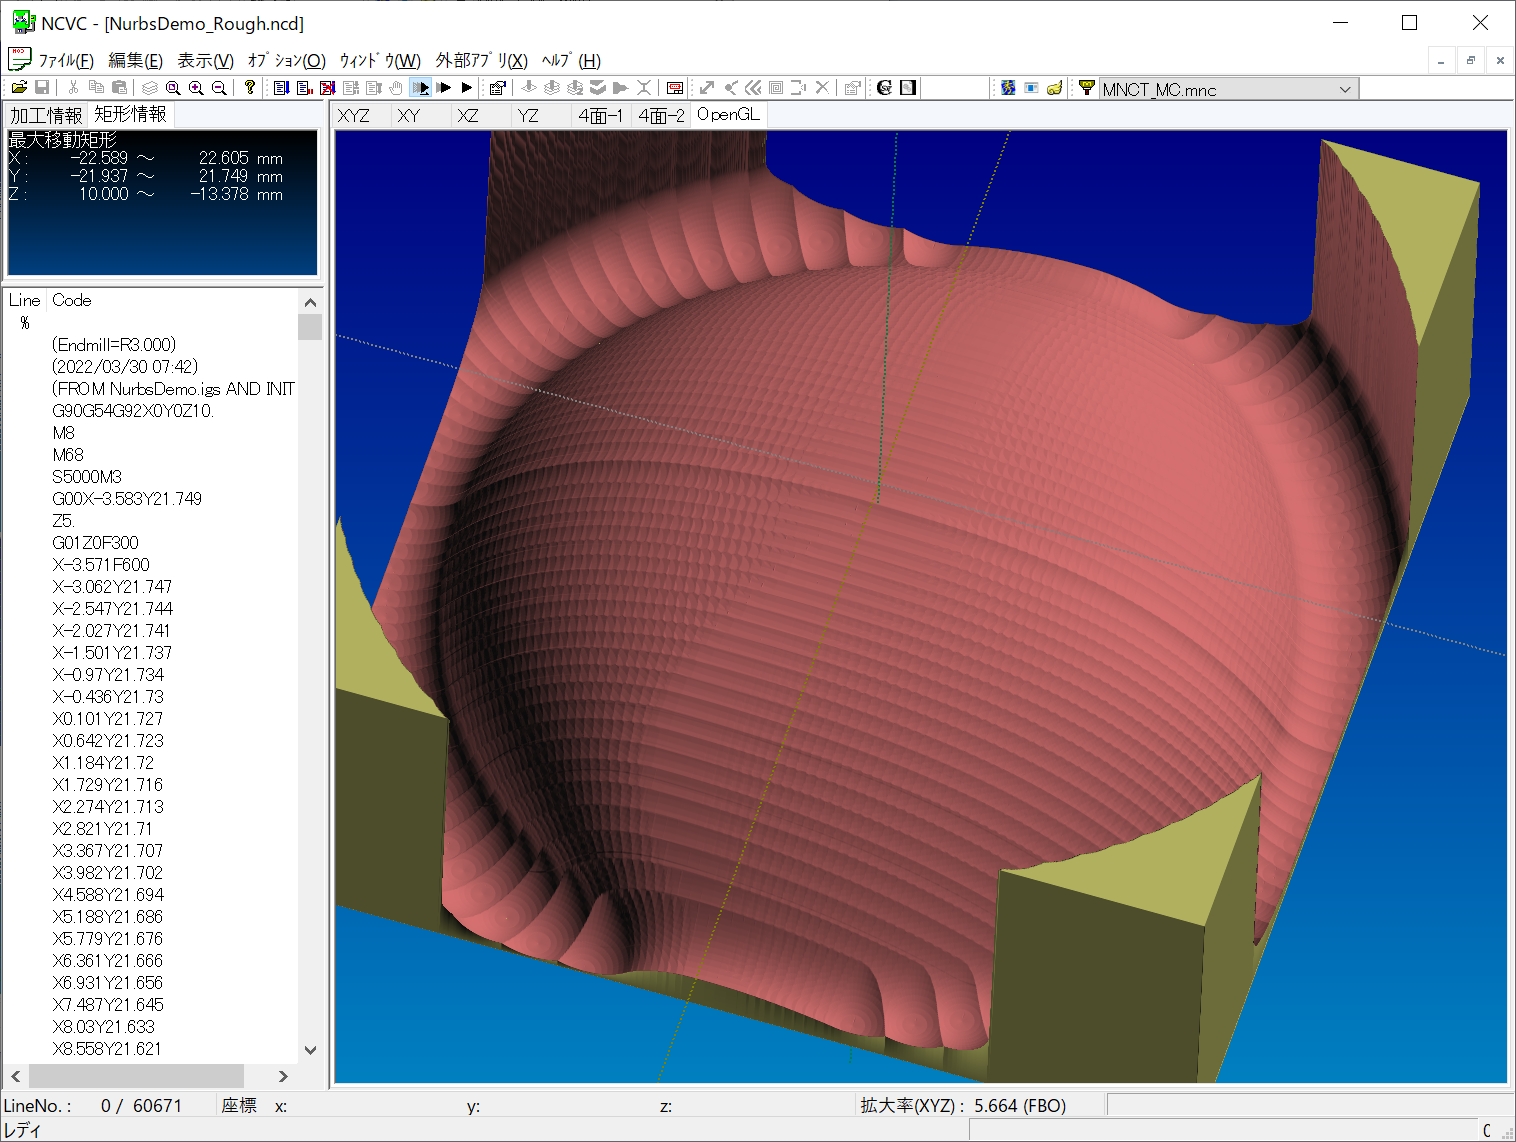
\includegraphics[scale=0.5]{No2/fig/fig29.png}
\caption{荒加工NCデータのシミュレーション結果Ⅱ}
\label{fig:ncvc29}
\end{figure}
